 
\chapter{Applications of the Frisch--Waugh--Lovell Theorem}\label{chapter::FWL-application}
 
The FWL theorem has many applications, and I will highlight some of them in
this chapter. 



\section{Centering regressors}

As a special case, partition the covariate matrix into $X=(X_1,X_2)$ with  $X_{1}=1_{n}$. This is the usual case including the constant as the first regressor.   
The projection matrix 
\[
H_{1}=1_{n}(1_{n}^{\T}1_{n})^{-1}1_{n}^{\T} 
=n^{-1}1_{n}1_{n}^{\T} = \begin{pmatrix}
n^{-1} & \cdots & n^{-1} \\
\vdots && \vdots \\
n^{-1} &\cdots & n^{-1} 
\end{pmatrix} \equiv A_n
\]
 contains $n^{-1}$'s as its elements, and 
 $$
 C_{n}=I_{n}-n^{-1}1_{n}1_{n}^{\T}
 $$
is the projection matrix orthogonal to $1_{n}$. Multiplying any vector by $A_n$ is equivalent to obtaining the average of its components, and multiplying any vector 
by $C_{n}$ is equivalent to centering that vector, for example, 
\[
A_n Y = \left(\begin{array}{c}
 \bar{y}\\
\vdots\\
 \bar{y}
\end{array}\right) =  \bar{y} 1_n ,
\]
and
\[
C_{n}Y=\left(\begin{array}{c}
y_{1}-\bar{y}\\
\vdots\\
y_{n}-\bar{y}
\end{array}\right).
\]
More generally, multiplying any matrix by $A_n$ is equivalent to averaging each column, and multiplying any matrix by $C_{n}$ is equivalent to centering each
column of that matrix, for example,
\[
A_n X_2 = \left(\begin{array}{c}
 \bar{x}_{2}^{\T}\\
\vdots\\
 \bar{x}_{2}^{\T}
\end{array}\right) = 1_n  \bar{x}_{2}^{\T} , 
\]
and
\[
C_{n}X_{2}=\left(\begin{array}{c}
x_{12}^{\T}-\bar{x}_{2}^{\T}\\
\vdots\\
x_{n2}^{\T}-\bar{x}_{2}^{\T}
\end{array}\right),
\]
where $X_{2}$ contains row vectors $x_{12}^{\T},\ldots,x_{n2}^{\T}$ with average $\bar{x}_2 = n^{-1} \sumn x_{i2}$. The FWL
theorem implies that the coefficient of $X_2$ in the OLS fit of $Y$ on $(1_{n},X_{2})$ equals the coefficient of $C_{n}X_{2}$ 
 in the OLS fit of $C_{n}Y$ on $C_{n}X_{2}$,
that is, the OLS fit of the centered response vector on the column-wise
centered $X_{2}.$ An immediate consequence is that if each column is centered in the design matrix, then to obtain the OLS coefficients, it does not matter whether to
include the column $1_{n}$ or not. 

The centering matrix $C_{n}$ has another property: its quadratic
form equals the sample variance multiplied by $n-1$, for example,
\begin{eqnarray*}
Y^{\T}C_{n}Y&=&Y^{\T} C_{n}^{\T} C_{n}Y \\
&=& (y_{1}-\bar{y},\ldots, y_{n}-\bar{y})  \left(\begin{array}{c}
y_{1}-\bar{y}\\
\vdots\\
y_{n}-\bar{y}
\end{array}\right) \\
&=& \sumn(y_{i}-\bar{y})^{2} \\
&=& (n-1) \hat{\sigma}^2_y,
\end{eqnarray*}
where $ \hat{\sigma}^2_y $ is the sample variance of the outcomes. 
For an $n\times p$ matrix $X$, 
\begin{align*}
X^{\T}C_{n}X 
%& =X^{\T}(I_{n}-n^{-1}1_{n}1_{n}^{\T})X\\
 & =\left(\begin{array}{c}
X_{1}^{\T}\\
\vdots\\
X_{p}^{\T}
\end{array}\right) C_{n}  \left(\begin{array}{ccc}
X_{1} & \cdots & X_{p}\end{array}\right)\\
&= \left(\begin{array}{ccc}
X_1^{\T} C_n X_1 & \cdots & X_1^{\T} C_n X_p \\
\vdots &  & \vdots\\
X_p^{\T} C_n X_1  & \cdots & X_p^{\T} C_n X_p 
\end{array}\right) \\ 
 & =(n-1)\left(\begin{array}{ccc}
\hat{\sigma}_{11} & \cdots & \hat{\sigma}_{1p}\\
\vdots &  & \vdots\\
\hat{\sigma}_{p1} & \cdots & \hat{\sigma}_{pp}
\end{array}\right),
\end{align*}
where 
$$
\hat{\sigma}_{j_{1}j_{2}}=(n-1)^{-1}\sumn(x_{ij_{1}}-\bar{x}_{\cdot j_{1}})(x_{ij_{2}}-\bar{x}_{\cdot j_{2}})
$$
is the sample covariance between $X_{j_{1}}$ and $X_{j_{2}}$. 
So $(n-1)^{-1} X^{\T} C_n X$ equals the sample covariance matrix of $X$. 
For these reason, I choose the notation $C_n$ with ``$C$'' for both ``centering'' and ``covariance.'' 

In another important special case, $X_{1}$ contains the dummies for
a discrete variable, for example, the indicators for different treatment
levels or groups. 
See Example \ref{eg::anova-H} for the background. 
With $k$ groups, $X_{1}$ can take the following
two forms:
\begin{eqnarray}\label{eq::discrete-regressor-dummy}
X_{1}=\left(\begin{array}{cccc}
1 & 1 & \cdots & 0\\
\vdots & \vdots &  & \vdots\\
1 & 1 & \cdots & 0\\
\vdots & \vdots &  & \vdots\\
1 & 0 & \cdots & 1\\
\vdots & \vdots &  & \vdots\\
1 & 0 &  & 1\\
1 & 0 &  & 0\\
\vdots & \vdots &  & \vdots\\
1 & 0 & \cdots & 0
\end{array}\right)_{n\times k}\qquad\text{or}\qquad X_{1}=\left(\begin{array}{ccc}
1 & \cdots & 0\\
\vdots &  & \vdots\\
1 & \cdots & 0\\
\vdots &  & \vdots\\
0 & \cdots & 1\\
\text{\ensuremath{\vdots}} &  & \vdots\\
0 & \cdots & 1
\end{array}\right)_{n\times k},
\end{eqnarray}
where the first form of $X_1$ contains $1_{n}$ and $k-1$ dummy variables,
and the second form of $X_1$ contains $k$ dummy variables. In both forms
of $X_{1}$, the observations are sorted according to the group indicators.
If we regress $Y$ on $X_{1}$, the residual vector is 
\begin{eqnarray}\label{eq::centeringbyK}
Y - 
\left(\begin{array}{c}
 \bar{y}_{[1]}\\
\vdots\\
 \bar{y}_{[1]}\\
\vdots\\
 \bar{y}_{[k]}\\
\vdots\\
 \bar{y}_{[k]}
\end{array}\right),
\end{eqnarray}
where $\bar{y}_{[1]},\ldots,\bar{y}_{[k]}$ are the averages of the
outcomes within groups $1,\ldots,k$. Effectively, we center $Y$ by
group-specific means. Similarly, if we regress $X_{2}$ on $X_{1}$,
we center each column of $X_{2}$ by the group-specific means. Let
$Y^{\textsc{c}}$ and $X_{2}^{\textsc{c}}$ be the centered response
vector and design matrix. The FWL theorem implies that the OLS coefficient
of $X_{2}$ in the long regression is the OLS coefficient of $X_{2}^{\textsc{c}}$
in the partial regression of $Y^{\textsc{c}}$ on $X_{2}^{\textsc{c}}$.
When $k$ is large, running the OLS with centered variables can reduce
the computational cost. 




\section{Partial correlation coefficient and Simpson's paradox\label{sec:Partial-correlation-coefficient}}

The sample Pearson correlation coefficient between $n$ observations of two
scalars $(x_{i},y_{i})_{i=1}^n $
\[
 \hat{\rho}_ {yx}=\frac{\sumn(x_{i}-\bar{x})(y_{i}-\bar{y})}{\sqrt{\sumn(x_{i}-\bar{x})^{2}}\sqrt{\sumn(y_{i}-\bar{y})^{2}}}
\]
measures the linear relationship between $x$ and $y$. How do we
measure the linear relationship between $x$ and $y$ after controlling
for some other variables $w\in\mathbb{R}^{k-1}$? Intuitively, we
can measure it with the sample Pearson correlation coefficient based on the
residuals from the following two OLS fits:
\begin{enumerate}
[(R1)]
\item \label{enu:partialols1}run OLS of $Y$ on $(1,W)$ and obtain residual
vector $\hat{\varepsilon}_{y}$ and residual sum of squares $\textsc{rss}_{y}$;
\item \label{enu:partialols2}run OLS of $X$ on $(1,W)$ and obtain residual
vector $\hat{\varepsilon}_{x}$ and residual sum of squares $\textsc{rss}_{x}$.
\end{enumerate}
%
With $\hat{\varepsilon}_{y}$ and $\hat{\varepsilon}_{x}$, we can
define the sampling partial correlation coefficient between $x$ and $y$ given
$w$ as 
\[
 \hat{\rho}_ {yx\mid w}=\frac{\sumn\hat{\varepsilon}_{x,i}\hat{\varepsilon}_{y,i}}{\sqrt{\sumn\hat{\varepsilon}_{x,i}^{2}}\sqrt{\sumn\hat{\varepsilon}_{y,i}^{2}}}.
\]
 In the above definition, we do not center the residuals because they
have zero sample means due to the inclusions of the intercept in the
OLS fits (R\ref{enu:partialols1}) and (R\ref{enu:partialols2}). The sample partial correlation coefficient determines the coefficient of $\hat{\varepsilon}_{x}$ in the OLS fit  of $\hat{\varepsilon}_{y}$ on $\hat{\varepsilon}_{x}$:
\begin{eqnarray}
\label{eq::galtonianformula-multiple}
\hat{\beta}_{yx\mid w}=\frac{\sumn\hat{\varepsilon}_{x,i}\hat{\varepsilon}_{y,i}}{\sumn\hat{\varepsilon}_{x,i}^{2}}= \hat{\rho}_ {yx\mid w}\sqrt{\frac{\sumn\hat{\varepsilon}_{y,i}^{2}}{\sumn\hat{\varepsilon}_{x,i}^{2}}}= \hat{\rho}_ {yx\mid w}\frac{\hat{\sigma}_{y \mid  w}}{\hat{\sigma}_{x \mid  w}},
\end{eqnarray}
where $\hat{\sigma}_{y \mid  w}^{2}=\textsc{rss}_{y}/(n-k)$ and
$\hat{\sigma}_{x \mid  w}^{2}=\textsc{rss}_{x}/(n-k)$ are the
variance estimators based on regressions (R\ref{enu:partialols1}) and
(R\ref{enu:partialols2}) motivated by the Gauss--Markov model.  Based on the FWL theorem, $\hat{\beta}_{yx\mid w}$
equals the OLS coefficient of $X$ in the long regression of $Y$
on $(1,X,W).$ Therefore,  \eqref{eq::galtonianformula-multiple} is the Galtonian formula for multiple regression, which is analogous to that for univariate regression \eqref{eq::galtonian-formula-1}. 

 
To investigate the relationship between $y$ and $x$, different researchers
may run different regressions. One may run OLS of $Y$ on $(1, X ,W)$, and the other may run OLS of $Y$ on $(1, X ,W')$,
where $W'$ is a subset of $W$. Let $\hat{\beta}_{yx\mid w}$ be
the coefficient of $X$ in the first regression, and let $\hat{\beta}_{yx\mid w'}$
be the coefficient of $X$ in the second regression. Mathematically,
it is possible that these two coefficients have different signs, which
is called {\it Simpson's paradox}\footnote{The usual form of Simpson's paradox is in terms of a $2\times 2\times 2$ table with all binary variables. Here we focus on the continuous version.}. It is a paradox because we expect both
coefficients to measure the ``impact'' of $X$ on $Y$. Because these two coefficients have the same signs as the partial
correlation coefficients $ \hat{\rho}_ {yx\mid w}$ and $ \hat{\rho}_ {yx\mid w'}$, Simpson's
paradox is equivalent to 
\[
 \hat{\rho}_ {yx\mid w} \hat{\rho}_ {yx\mid w'}<0.
\]
To simplify the presentation, we discuss the special case with $w'$
being an empty set. Simpson's
paradox is then equivalent to 
\[
 \hat{\rho}_ {yx\mid w} \hat{\rho}_ {yx}<0.
\]
The following theorem gives an expression linking $ \hat{\rho}_ {yx\mid w}$ and $ \hat{\rho}_ {yx}$. 


\begin{theorem}\label{thm::sample-partialcorr-corr}
For $Y,X,W\in\mathbb{R}^{n}$, we have 
\[
 \hat{\rho}_ {yx\mid w}=\frac{ \hat{\rho}_ {yx}- \hat{\rho}_ {yw} \hat{\rho}_ {xw}}{\sqrt{1- \hat{\rho}_ {yw}^{2}}\sqrt{1- \hat{\rho}_ {xw}^{2}}}.
\]
\end{theorem}
 
 
 
 
\begin{figure}
\centering
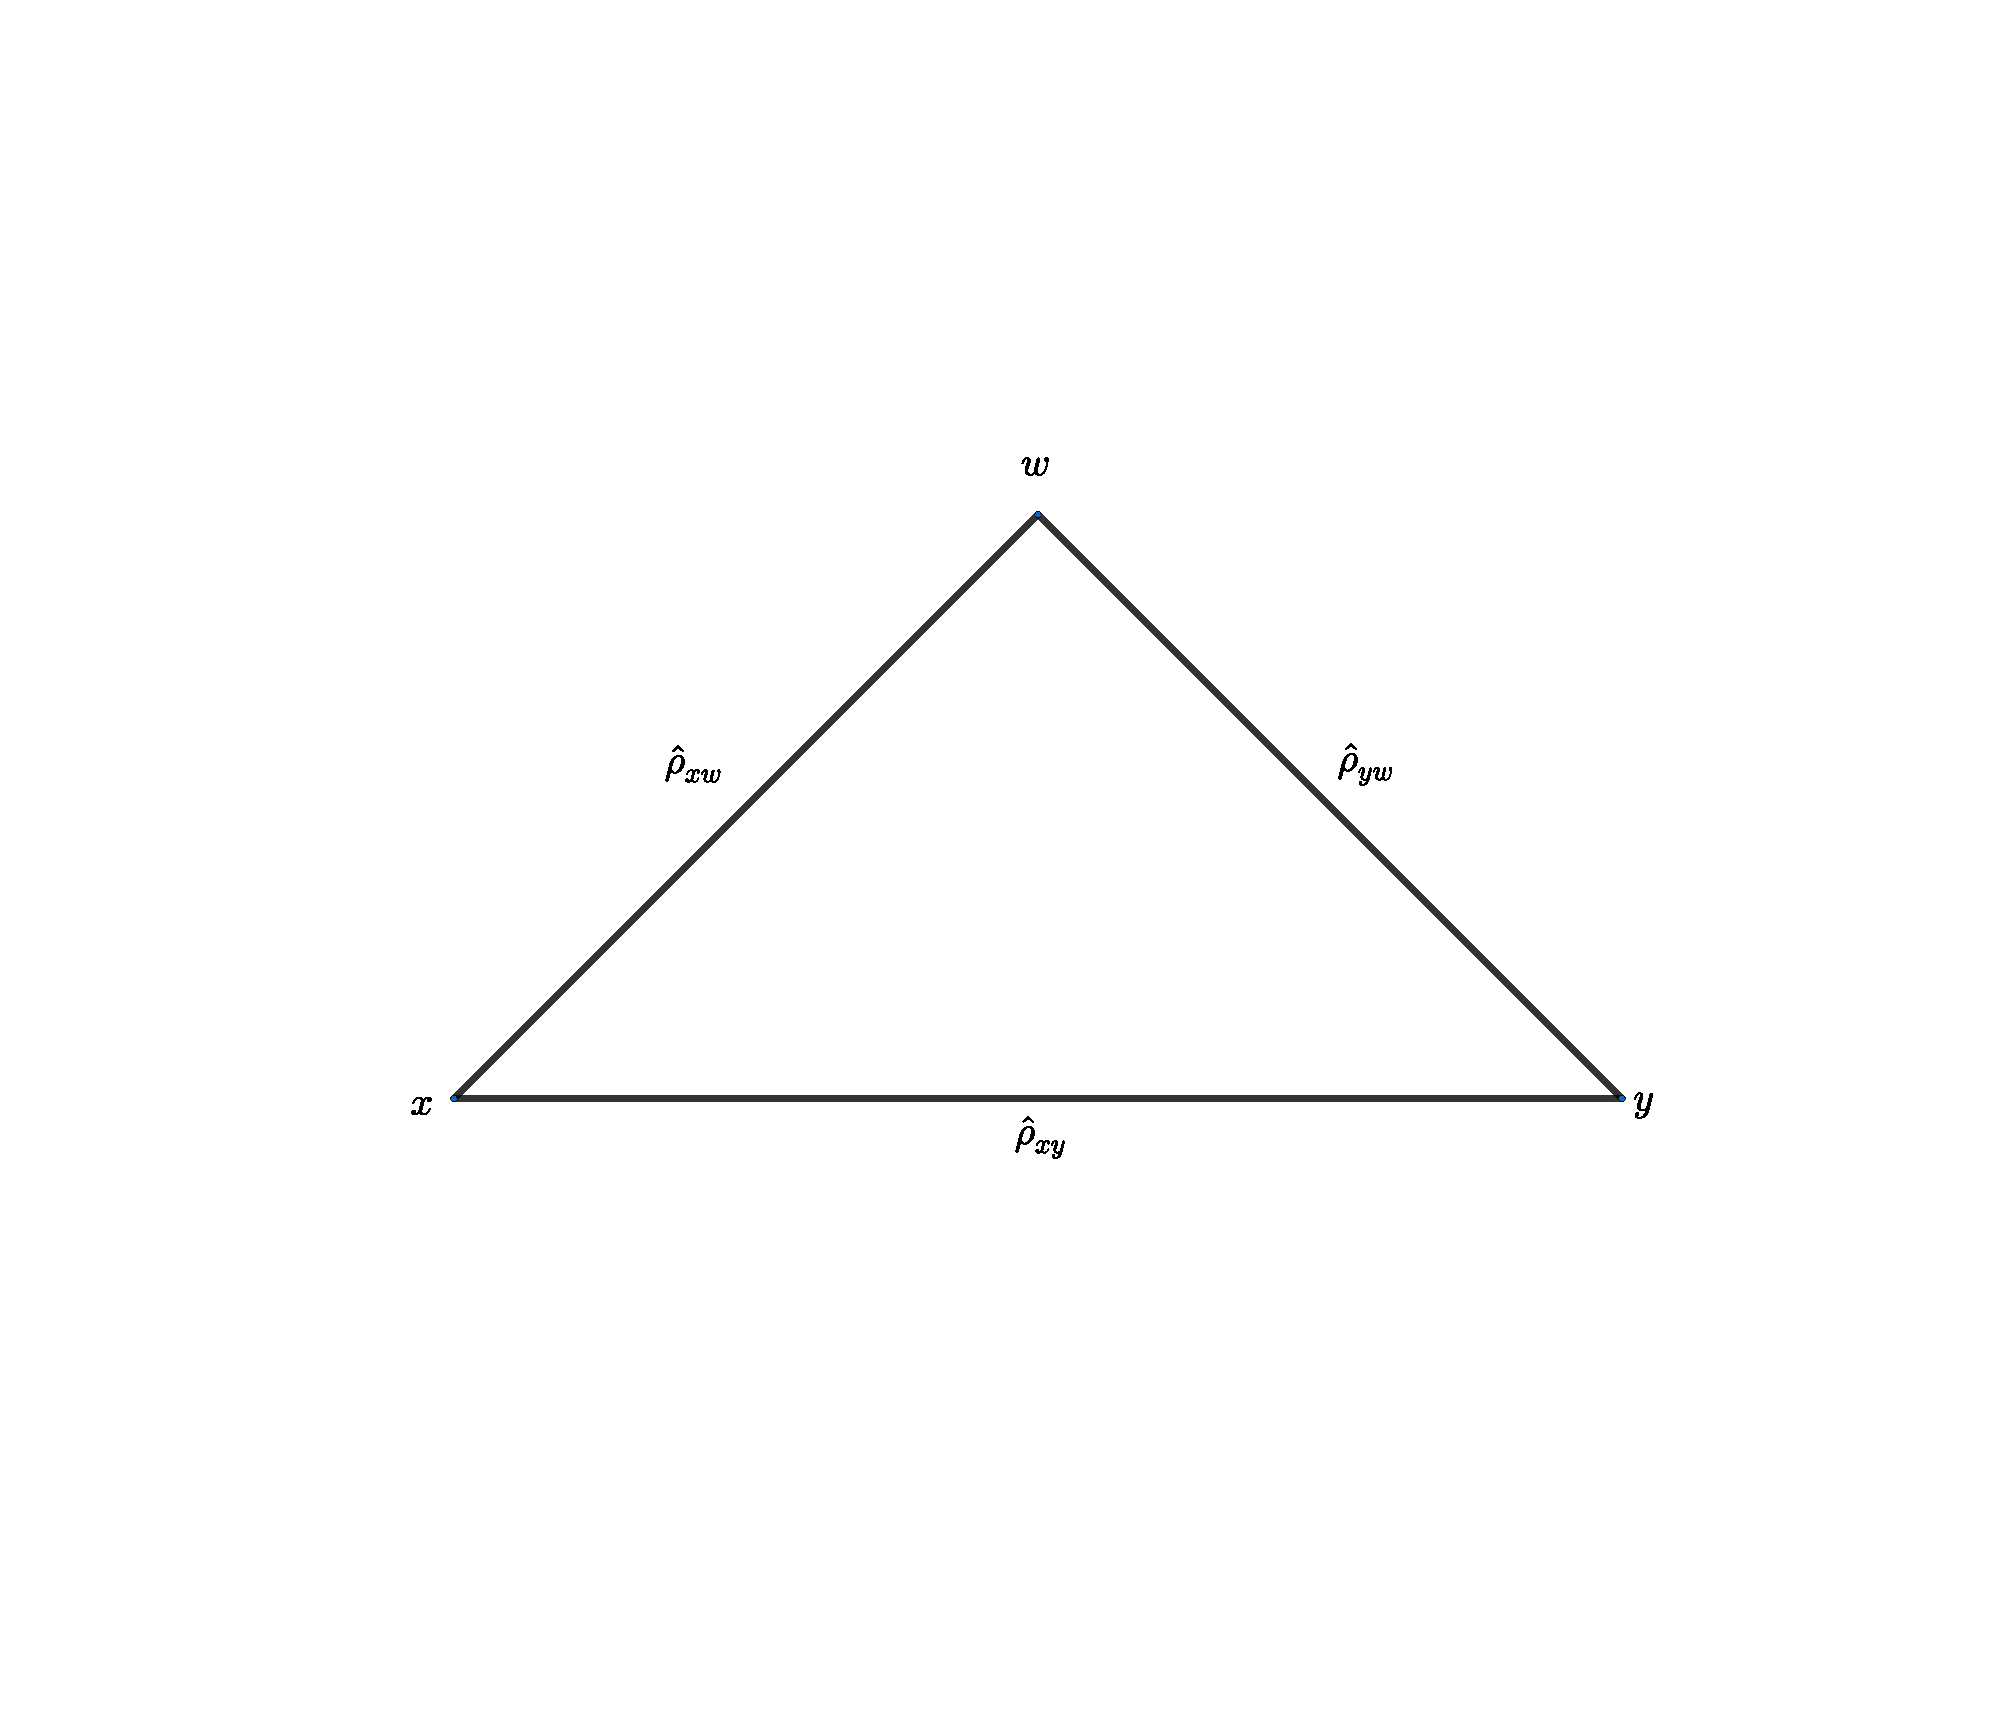
\includegraphics[width = 0.9\textwidth]{figures/partialcorrelationtriangle.pdf}
\caption{Correlations among three variables}\label{fig::correlations3}
\end{figure} 
 
 Its proof is purely algebraic, so I leave it as Problem \ref{hw7::sample-partial-correlation}. Theorem \ref{thm::sample-partialcorr-corr} states that we can obtain the sample partial correlation coefficient based on the three pairwise correlation coefficients. Figure \ref{fig::correlations3} illustrates the interplay among three variables. In particular, the correlation between $x$ and $y$ is due to two ``pathways'': the one acting through $w$ and the one acting independent of $w$. The first path way is related to the product term $ \hat{\rho}_ {yw} \hat{\rho}_ {xw}$, and the second pathway is related to $ \hat{\rho}_ {yx\mid w}$. This gives some intuition for Theorem \ref{thm::sample-partialcorr-corr}. 
 
 
Based on data $(y_{i},x_{i},w_{i})_{i=1}^{n}$, we can compute the
sample correlation matrix
\[
\hat{R}  =\left(\begin{array}{ccc}
1 &  \hat{\rho}_ {yx} &  \hat{\rho}_ {yw}\\
 \hat{\rho}_ {xy} & 1 &  \hat{\rho}_ {xw}\\
 \hat{\rho}_ {wy} &  \hat{\rho}_ {wx} & 1
\end{array}\right),
\]
which is symmetric and positive semi-definite. 
%Since $\hat{R}$ is $3\times3$
%and the $\hat{\rho}$'s are smaller than or equal to one, its positive semi-definiteness
%is equivalent to $\text{det}(\hat{R})\geq0$. With this only constraint,
Simpson's paradox happens if and only if
\[
 \hat{\rho}_ {yx}( \hat{\rho}_ {yx}- \hat{\rho}_ {yw} \hat{\rho}_ {xw})<0\Longleftrightarrow  \hat{\rho}_ {yx}^{2}< \hat{\rho}_ {yx} \hat{\rho}_ {yw} \hat{\rho}_ {xw}.
\]
 
 
We can observe Simpson's Paradox in the following simulation with the \ri{R} code in \ri{code8.2.R}. 


\begin{lstlisting}
> n  = 1000
> w  = rbinom(n, 1, 0.5)
> x1 = rnorm(n, -1, 1)
> x0 = rnorm(n, 2, 1)
> x  = ifelse(w, x1, x0)
> y  = x + 6*w + rnorm(n)
> fit.xw = lm(y ~ x + w)$coef
> fit.x  = lm(y ~ x)$coef
> fit.xw 
(Intercept)           x           w 
 0.05655442  0.97969907  5.92517072 
> fit.x 
(Intercept)           x 
  3.6422978  -0.3743368 
\end{lstlisting}


Because $w$ is binary, we can plot $(x,y)$ in each group of $w=1$ and $w=0$ in Figure \ref{fig::simpsonparadoxexample}. In both groups, $y$ and $x$ are positively associated with positive regression coefficients; but in the pooled data, $y$ and $x$ are negatively associated with a negative regression coefficient. 

\begin{figure}[ht]
\centering
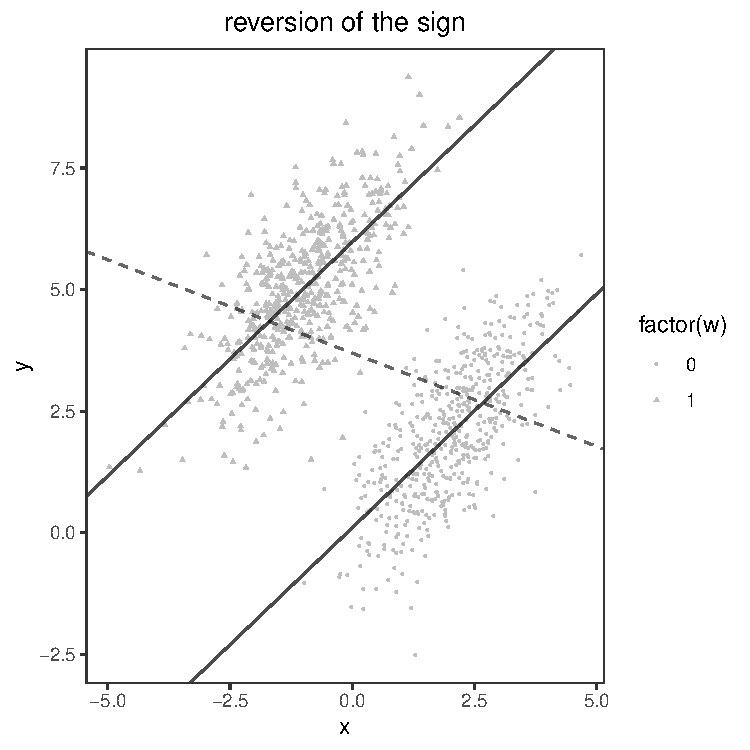
\includegraphics[width = 0.8\textwidth]{figures/simpsonparadoxexample_ggplot.pdf}
\caption{An Example of Simpson's Paradox. The two solid regression lines are fitted separately using the data from two groups, and the dash regression line is fitted using the pooled data. }\label{fig::simpsonparadoxexample}
\end{figure}
 
 

\section{Hypothesis testing and analysis of variance}\label{sec::fwl-anova}

Partition $X$ and $\beta$ into
\[
X=\left(\begin{array}{cc}
X_{1} & X_{2}\end{array}\right),\qquad\beta=\left(\begin{array}{c}
\beta_{1}\\
\beta_{2}
\end{array}\right),
\]
where $X_{1}\in\mathbb{R}^{n\times k},X_{2}\in\mathbb{R}^{n\times l},\beta_{1}\in\mathbb{R}^{k}$
and $ \beta_2 \in  \mathbb{R}^{l}.$ We are often interested in testing
\[
H_{0}:\beta_{2}=0
\]
in the long regression
\begin{equation}
Y=X\beta+\varepsilon=X_{1}\beta_{1}+X_{2}\beta_{2}+\varepsilon,\label{eq:longreg}
\end{equation}
where $\varepsilon\sim\N(0,\sigma^{2}I_{n}).$ If $H_{0}$ holds,
then $X_{2}$ is redundant and a short regression suffices:
\begin{equation}
Y=X_{1}\beta+\varepsilon. \label{eq:shortreg}
\end{equation}
This is a special case of testing $C\beta=0$
with 
\[
C=\left(\begin{array}{cc}
0_{l\times k} & I_{l\times l}\end{array}\right).
\]
As discussed before, we can use 
\[
\hat{\beta}_{2}\sim\N(0,\sigma^{2}S_{22})
\]
with $S_{22} = (\tilde{X}_{2}^{\T}\tilde{X}_{2})^{-1}$ being the $(2,2)$th block of $(X^{\T}X)^{-1}$ by Lemma \ref{lem:blockinverse}, to construct the Wald-type statistic for hypothesis testing:
\begin{eqnarray*}
F_{\text{Wald}}  
&=& \frac{\hat{\beta}_{2}^{\T}(S_{22})^{-1}\hat{\beta}_{2}}{l\hat{\sigma}^{2}}
\\
&=& \frac{\hat{\beta}_{2}^{\T}  \tilde{X}_{2}^{\T}\tilde{X}_{2}  \hat{\beta}_{2}}{l\hat{\sigma}^{2}}
\\
&\sim & F_{l,n-p}.
\end{eqnarray*}


Now I will discuss testing  $H_{0}$ from an alternative perspective based on comparing the residual sum of squares in the long regression (\ref{eq:longreg}) and the short regression (\ref{eq:shortreg}). This technique is called the analysis of variance (ANOVA), pioneered by R. A. Fisher in the design and analysis of experiments. Intuitively, if $\beta_{2}=0$, then the residual vectors from the long regression (\ref{eq:longreg})
and the short regression (\ref{eq:shortreg}) should not be ``too
different.'' However, with the error term $\varepsilon$, these residuals are
random, then the key is to quantify the magnitude of the difference.
Define 
\[
\textsc{rss}_{\text{long}}=Y^{\T}(I_{n}-H)Y
\]
and 
\[
\textsc{rss}_{\text{short}}=Y^{\T}(I_{n}-H_{1})Y
\]
as the residual sum of squares from the long and short regressions,
respectively. By the definition of OLS, it must be true that
$$
\textsc{rss}_{\text{long}}\leq\textsc{rss}_{\text{short}} 
$$
and
\begin{equation}
\textsc{rss}_{\text{short}}-\textsc{rss}_{\text{long}}
=Y^{\T}(H-H_{1})Y
\geq 0.\label{eq:diffvar}
\end{equation}
To understand the magnitude of the change in the residual sum of squares,
we can standardize the above difference and define
\[
F_\textsc{anova} = \frac{(\textsc{rss}_{\text{short}}-\textsc{rss}_{\text{long}})/l}{\textsc{rss}_{\text{long}}/(n-p)},
\]
In the definition of the above statistic, $l$ and $n-p$ are the
degrees of freedom to make the mathematics more elegant, but
they do not change the discussion fundamentally. The denominator of $F_\textsc{anova} $
is $\hat{\sigma}^{2}$, so we can also write it as 
\begin{equation}
F_\textsc{anova} =\frac{\textsc{rss}_{\text{short}}-\textsc{rss}_{\text{long}}}{l\hat{\sigma}^{2}}.\label{eq:Fformula}
\end{equation}


The following theorem states that these two perspectives yield an identical test statistic. 


\begin{theorem}\label{thm::f-two-proofs}
Under Assumption \ref{assume::nlm}, if $\beta_{2}=0$, then $F_\textsc{anova} \sim F_{l,n-p}.$
In fact, $F_\textsc{anova} =F_\text{Wald}  $ which is a numerical result without Assumption \ref{assume::nlm}. 
\end{theorem}



I divide the proof into two parts. The first part derives the exact distribution of $F_\textsc{anova}$ under the Normal linear model. It relies on the following lemma on the basic properties of the projection matrices. I relegate its proof to Problem \ref{problem07::projection-matrices}. 

\begin{lemma}\label{lemma::projection-m-F}
We have
$$
HX_{1}=X_{1}, \quad HX_2 = X_2, \quad  HH_{1} =H_{1},\quad H_{1}H=H_{1}
$$
Moreover, 
$H-H_{1}$ is a projection matrix of rank $p-k=l$, 
$I_{n}-H$ is a projection matrix of rank $n-p$, and they are orthogonal:
\begin{equation}
(H-H_{1})(I_{n}-H)=0.\label{eq:basic4}
\end{equation}
\end{lemma}

\begin{myproof}{Theorem}{\ref{thm::f-two-proofs} (Part I)}
%The proof has two steps. 
%\paragraph*{Step 1.} I will prove the distribution of $F_\textsc{anova} $ directly. 
%First, I will
%use the following basic facts repeatedly:
%\begin{align}
%HX & =X\Longrightarrow H\left(\begin{array}{cc}
%X_{1} & X_{2}\end{array}\right)=\left(\begin{array}{cc}
%X_{1} & X_{2}\end{array}\right)\Longrightarrow HX_{1}=X_{1},\label{eq:basic1}\\
%HH_{1} & =H_{1},\qquad H_{1}H=H_{1},\label{eq:basic2}\\
%(H-H_{1})X_{1} & =0;\label{eq:basic3}
%\end{align}
%$H-H_{1}$ is a projection matrix of rank $p-k=l$, 
%$I_{n}-H$ is a projection matrix of rank $n-p$, and they are orthogonal:
%\begin{equation}
%(H-H_{1})(I_{n}-H)=0.\label{eq:basic4}
%\end{equation}
%I leave it as a homework problem to verify these. 

The residual vector from the long regression is $\hat{\varepsilon}=(I_{n}-H)Y=(I_{n}-H)(X\beta+\varepsilon)=(I_{n}-H)\varepsilon$,
so the residual sum of squares is 
\[
\textsc{rss}_{\text{long}}=\hat{\varepsilon}^{\T}\hat{\varepsilon}=\varepsilon^{\T}(I_{n}-H)\varepsilon;
\]
since $\beta_{2}=0$, the residual vector from the short regression
is $\tilde{\varepsilon}=(I_{n}-H_{1})Y=(I_{n}-H_{1})(X_{1}\beta_{1}+\varepsilon)=(I_{n}-H_{1})\varepsilon$,
so the residual sum of squares is
\[
\textsc{rss}_{\text{short}}=\tilde{\varepsilon}^{\T}\tilde{\varepsilon}=\varepsilon^{\T}(I_{n}-H_{1})\varepsilon.
\]
Let $\varepsilon_{0}=\varepsilon/\sigma\sim\N(0,I_{n})$ be a standard
Normal random vector, then we can write $F_\textsc{anova} $ as
\begin{eqnarray}
F_\textsc{anova}  &=& \frac{\varepsilon^{\T}(H-H_{1})\varepsilon/l}{\varepsilon^{\T}(I_{n}-H)\varepsilon/(n-p)} \nonumber  \\
&=&\frac{\varepsilon_{0}^{\T}(H-H_{1})\varepsilon_{0}/l}{\varepsilon_{0}^{\T}(I_{n}-H)\varepsilon_{0}/(n-p)} \nonumber\\
&=&\frac{\|(H-H_{1})\varepsilon_{0}\|^{2}/l}{\|(I_{n}-H)\varepsilon_{0}\|^{2}/(n-p)}.\label{eq:FratioofQ}
\end{eqnarray}

Therefore, we have the following joint Normality using the basic fact
(\ref{eq:basic4}): 
\begin{align*}
\left(\begin{array}{c}
(H-H_{1})\varepsilon_{0}\\
(I_{n}-H)\varepsilon_{0}
\end{array}\right) & =\left(\begin{array}{c}
H-H_{1}\\
I_{n}-H
\end{array}\right)\varepsilon_{0}\\
 & \sim\N\left\{ \left(\begin{array}{c}
0\\
0
\end{array}\right),\left(\begin{array}{cc}
H-H_{1} & 0\\
0 & I_{n}-H
\end{array}\right)\right\} .
\end{align*}
So $(H-H_{1})\varepsilon_{0}$ and $(I_{n}-H)\varepsilon_{0}$ are
Normal with mean zero and two projection matrices $H-H_{1}$ and $I_{n}-H$
as covariances, respectively, and moreover, they are independent.
These imply that their squared lengths are chi-squared:
\[
\|(H-H_{1})\varepsilon_{0}\|^{2}\sim\chi_{l}^{2},\qquad\|(I_{n}-H)\varepsilon_{0}\|^{2}\sim\chi_{n-p}^{2},
\]
and they are independent. These facts, coupled with (\ref{eq:FratioofQ}),
imply that $F_\textsc{anova}  \sim F_{l,n-p}.$ 
\end{myproof}


The second part demonstrates that $F_\textsc{anova}  = F_\text{Wald}$ without assuming the Normal linear model, which gives an indirect proof for the exact distribution of $F_\textsc{anova}$ under the Normal linear model. 

\begin{myproof}{Theorem}{\ref{thm::f-two-proofs} (Part II)}
%\paragraph*{Step 2.} I will show that $F_\textsc{anova}  = F_\text{Wald}$ which gives an indirect proof for
%the distribution of $F_\textsc{anova} .$ 
Using the FWL theorem that $\hat{\beta}_{2}=(\tilde{X}_{2}^{\T}\tilde{X}_{2})^{-1}\tilde{X}_{2}^{\T}Y$,
%and the fact that $S_{22}=(\tilde{X}_{2}^{\T}\tilde{X}_{2})^{-1}$,
we can rewrite $F_\text{Wald} $ as 
\begin{align}
F_\text{Wald} & =\frac{Y^{\T}\tilde{X}_{2}(\tilde{X}_{2}^{\T}\tilde{X}_{2})^{-1}\tilde{X}_{2}^{\T}\tilde{X}_{2}(\tilde{X}_{2}^{\T}\tilde{X}_{2})^{-1}\tilde{X}_{2}^{\T}Y}{l\hat{\sigma}^{2}}\nonumber \\
 & =\frac{Y^{\T}\tilde{X}_{2}(\tilde{X}_{2}^{\T}\tilde{X}_{2})^{-1}\tilde{X}_{2}^{\T}Y}{l\hat{\sigma}^{2}}\nonumber \\
 & =\frac{Y^{\T}\tilde{H}_{2}Y}{l\hat{\sigma}^{2}},\label{eq:Wformula}
\end{align}
recalling that  
$
\tilde{H}_{2}=\tilde{X}_{2}(\tilde{X}_{2}^{\T}\tilde{X}_{2})^{-1}\tilde{X}_{2}^{\T}
$
is the projection matrix onto the column space of $\tilde{X}_{2}.$ Therefore, $F_\textsc{anova}  = F_\text{Wald}$ follows from the basic identity $H-H_{1}=\tilde{H}_{2}$ ensured by Lemma \ref{lemma::decompose-projection-matrices}. 
\end{myproof}
 
 
We can use the \ri{anova} function in \ri{R} to compute the $F$ statistic and the $p$-value. Below I revisit the \ri{lalonde} data with the \ri{R} code in \ri{code8.3.R}.  The result is identical as in Section \ref{section::normal-lm-lalonde}. 


 \begin{lstlisting}
> library("Matching")
> data(lalonde)
> lalonde_full  = lm(re78 ~ ., data = lalonde)
> lalonde_treat = lm(re78 ~ treat, data = lalonde)
> anova(lalonde_treat, lalonde_full)
Analysis of Variance Table

Model 1: re78 ~ treat
Model 2: re78 ~ age + educ + black + hisp + married + nodegr + re74 + 
    re75 + u74 + u75 + treat
  Res.Df        RSS Df Sum of Sq      F  Pr(>F)  
1    443 1.9178e+10                              
2    433 1.8389e+10 10 788799023 1.8574 0.04929 *
\end{lstlisting}


In fact, we can conduct an analysis of variance in a sequence of models. For example, we can supplement the above analysis with a model containing only the intercept. The function \ri{anova} works for a sequence of nested models with increasing complexities. 
\begin{lstlisting}
> lalonde1   = lm(re78 ~ 1, data = lalonde)
> anova(lalonde1, lalonde_treat, lalonde_full)
Analysis of Variance Table

Model 1: re78 ~ 1
Model 2: re78 ~ treat
Model 3: re78 ~ age + educ + black + hisp + married + nodegr + re74 + 
    re75 + u74 + u75 + treat
  Res.Df        RSS Df Sum of Sq      F   Pr(>F)   
1    444 1.9526e+10                                
2    443 1.9178e+10  1 348013456 8.1946 0.004405 **
3    433 1.8389e+10 10 788799023 1.8574 0.049286 * 
\end{lstlisting}

Overall, the treatment variable is significantly related to the outcome but none of the pretreatment covariate is. 

 






\section{Homework problems}

\paragraph{FWL with intercept}\label{hw7::fwl-intercept}

The following result is an immediate extension of Theorem \ref{thm:fwl}.  

Partition $X$ and $\beta$ into
\[
X=\left(\begin{array}{ccc}
1_n & X_{1} & X_{2}\end{array}\right),\qquad
\beta=\left(\begin{array}{c}
\beta_0 \\
\beta_{1}\\
\beta_{2}
\end{array}\right),
\]
where $X_{1}\in\mathbb{R}^{n\times k},X_{2}\in\mathbb{R}^{n\times l},  \beta_0 \in \mathbb{R},  \beta_{1}\in\mathbb{R}^{k}$ and $\beta_2 \in  \mathbb{R}^{l}$.  then we can consider the {\it long regression} 
\begin{eqnarray*}
Y &=& X\hat{\beta}+\hat{\varepsilon} \\
&=& \left(\begin{array}{ccc}
1_n & X_{1} & X_{2}\end{array}\right)\left(\begin{array}{c}
\hat{\beta}_0 \\
\hat{\beta}_{1}\\
\hat{\beta}_{2}
\end{array}\right)+\hat{\varepsilon} \\
&=& 1_n \hat{\beta}_0 +  X_{1}\hat{\beta}_{1}+X_{2}\hat{\beta}_{2}+\hat{\varepsilon},
\end{eqnarray*}
 and the {\it short regression} 
\[
Y= 1_n \tilde{\beta}_0  +   X_{2}\tilde{\beta}_{2}+\tilde{\varepsilon},
\]
where $\hat{\beta}=\left(\begin{array}{c}
\hat{\beta}_0 \\ 
\hat{\beta}_{1}\\
\hat{\beta}_{2}
\end{array}\right)$ and
$
\left(\begin{array}{c}
\tilde{\beta}_{0}\\
\tilde{\beta}_{2}
\end{array}\right)
$ are the OLS coefficients, and $\hat{\varepsilon}$
and $\tilde{\varepsilon}$ are the residual vectors from the long
and short regressions, respectively. 

Prove the following theorem.

\begin{theorem}
\label{thm:fwl2}The OLS estimator for $\beta_{2}$ in the long regression equals the coefficient of $\tilde{X}_{2}$ in the OLS fit of $Y$ on $(1_n,\tilde{X}_{2} )$, where $\tilde{X}_{2}$ is the residual matrix of the column-wise OLS fit of $X_2$ on $(1_n, X_1)$, and also equals the coefficient of $\tilde{X}_{2}$ in the OLS fit of $\tilde{Y}$ on $(1_n,\tilde{X}_{2} )$, where $\tilde{Y}$ is the residual vector of the OLS fit of $Y$ on $(1_n, X_1)$.
\end{theorem}



\paragraph{General centering}\label{hw7::general-centering}

Verify \eqref{eq::centeringbyK}. 




\paragraph{Two-way centering of a matrix}\label{hw7::2way-centering}


Given $X \in \mathbb{R}^{n\times p}$, show that all rows and columns of $ C_n X C_p $ have mean $0$, where $C_n = I_n - n^{-1} 1_n 1_n^{\T}$ and  $C_p = I_p - p^{-1} 1_p 1_p^{\T}$. 



\paragraph{$t$-statistic in multivariate OLS}
\label{hw7::tstat-partialcorr-OLS}

This problem extends Problem \ref{hw5::t-ratio-univariateOLS}.


Focus on multivariate OLS discussed in Chapter \ref{chapter::normal-linear-model}: $y_i = \hat{\alpha}  +  \hat{\beta}_1 x_{i1} + \hat{\beta}_2^{\T} x_{i2} +  \hat{\varepsilon}_i$ $(i=1,\ldots, n)$, where $x_{i1}$ is a scalar and $x_{i2}$ can be a vector.  
Show that under homoskedasticity, the $t$-statistic associated with $ \hat{\beta}_1$ equals
$$
\frac{  \hat{\rho}_{yx_1|x_2}   }{  \sqrt{    (1  -  \hat{\rho}_{yx_1|x_2} ^2) /(n-p)  }   },
$$
where $p$ is the total number of regressors and $\hat{\rho}_{yx_1|x_2}$ is the sample partial correlation coefficient between $y$ and $x_1$ given $x_2$. 



Remark: \citet{frank2000impact} applied this formula to causal inference. 





\paragraph{Equivalence of the $t$-statistics in multivariate OLS}\label{hw7::t-stat-equivalent-multivariateOLS}


This problem extends Problems \ref{hw5::t-stat-equivalent} and \ref{hw6::t-stat-equivalent-breakdown}.  



With the data $(x_{i1}, x_{i2}, y_i)_{i=1}^n$ where both $x_{i1}$ and $y_i$ are scalars and $x_{i2}$ can be a vector. Run OLS fit of $y_i$ on $(1,x_{i1}, x_{i2})$ to obtain $t_{y\mid x_1, x_2}$, the $t$-statistic of the coefficient of $x_{i1}$, under the homoskedasticity assumption. Run OLS fit of $x_{i1}$ on $(1, y_i, x_{i2})$ to obtain $t_{x_1\mid y, x_2}$, the $t$-statistic of the coefficient of $y_i$, under the homoskedasticity assumption. 

Show $t_{y\mid x_1, x_2} = t_{x_1\mid y, x_2} $. Give a counterexample in which the numerical equivalence of the $t$-statistics breaks down based on the EHW standard error. 

 








\paragraph{Formula of the partial correlation coefficient}\label{hw7::sample-partial-correlation}

Prove Theorem \ref{thm::sample-partialcorr-corr}. 

\paragraph{Examples of Simpson's Paradox}

Give three numerical examples of $(Y,X,W)$ which causes Simpson's Paradox. Report the mean and covariance matrix for each example. 


\paragraph{Simpson's Paradox in reality}

Find a real-life dataset with Simpson's Paradox. 


\paragraph{Basic properties of projection matrices}\label{problem07::projection-matrices}
 
Prove Lemma \ref{lemma::projection-m-F}. 





\paragraph{Correlation of the regression coefficients}\label{hw::7:corr-reg-coef}


\begin{enumerate}
\item
Regress $Y$ on $(1_n,X_1, X_2)$ where $X_1$ and $X_2$ are two $n$-vectors with positive sample Pearson correlation $\hat\rho_{x_1x_2} > 0$. Show that the corresponding OLS coefficients $\hat{\beta}_1$ and $\hat{\beta}_2$ are negatively correlated under the Gauss--Markov model.

\item
Regress $Y$ on $(1_n,X_1, X_2, X_3)$ where $X_1$ and $X_2$ are two $n$-vectors and $X_3$ is an $n\times L$ dimensional matrix. If the partial correlation coefficient between $X_1$ and $X_2$ given $X_3$ is positive, then show that the corresponding OLS coefficients $\hat{\beta}_1$ and $\hat{\beta}_2$ are negatively correlated under the Gauss--Markov model.
\end{enumerate}




\paragraph{Inverse of sample covariance matrix and partial correlation coefficient}\label{hw::7:inverse-samplecov-pcc}

This is the sample version of Problem \ref{hwmath2::inverse-cov-conind-normal}.


Based on $X \in \mathbb{R}^{n\times p}$, we can compute the sample covariance matrix $\hat\Sigma$. Denote its inverse by $\hat\Sigma^{-1} = (\hat{\sigma}^{jk})_{1\leq j,k\leq p}$. Show that for any pair $j\neq k$, we have 
$$
\hat{\sigma}^{jk} = 0 \Longleftrightarrow \hat{\rho}_{x_jx_k\mid x_{\backslash (j,k)}} = 0
$$
where $\hat{\rho}_{x_jx_k\mid x_{\backslash (j,k)}} $ is the partial correlation coefficient of $X_j$ and $X_k$ given all other variables. 


